\section{Background}

This chapter describes the motivating application along with the Region Templates Framework, in which this work is developed, and some basic concepts of sensitivity analysis and computation reuse. Being the contributions of this work restricted to computation reuse, this chapter then ends with the analysis of some relevant related work on the subject.

\subsection{Microscopy Image Analysis}

It is now possible for biomedical researchers to capture highly detailed images from whole slide tissue samples in a few minutes with high-end microscopy scanners, which are becoming evermore available. This capability of collecting thousands of images on a daily basis extends the possibilities for generating detailed databases of several diseases. Through the investigation of tissue morphology of whole slide tissue images (WSI) there is the possibility of better understanding disease subtypes and feature distributions, enabling the creation of novel methods for classification of diseases. With the increasing number of research groups working and developing richer methods for carrying out quantitative microscopy image analyses \cite{micro1, micro2, micro3, micro4, micro5, micro6, micro7, micro8} and also the increasingly availability of digital microscopy imagery equipment, there is a high demand for systems or frameworks oriented towards the efficient execution of microscopy image analysis workflows.

% Biopsied tissue contains visual information that manifests from various molecular
% interactions that arise from disease and/or therapy. Microscopic examination
% of the tissue reveals this information enabling the pathologist to render
% accurate diagnoses, assess response and guide therapy. Whole slide digital
% imaging enables this process to be performed using digital images instead of
% physical slides. The quantitative characterization of microscopy image data
% involves a process of correcting for staining and imaging artifacts, systematic
% extraction and characterization of image features, detection of microanatomic
% objects, computing and characterizing their morphologic and molecular features,
% and monitoring and quantifying changes over space and time. In some imaging
% studies, processing also includes 3-D and/or spatio-temporal reconstruction.
% Each operation produces data products that can be directly consumed by client
% applications. In addition, operations can be combined together in a variety of
% ways to create additional data products or improve analysis results.

\begin{figure}[b]
\begin{center}

\includegraphics[width=1\textwidth]{img/nucleiPipelineCur.png}
\caption{An example microscopy image analysis workflow performed before image classification. Image extracted from \cite{barreiros_parallel_2017}.}
\label{fig:wf}
\end{center}
\end{figure}

The microscopy image analysis workflow used on this work is presented in Figure \ref{fig:wf} and was proposed by \cite{kong2013machine,DBLP:conf/bibm/KongWTCMKPSB13,Teodoro-IPDPS2013}. This workflow consists of normalization (1), segmentation (2), feature computation (3) and final classification (4), being the first three analysis stages the most computationally expensive phases. The first stage is responsible for normalizing the staining and/or illumination conditions of the image. The segmentation is the process of identifying the nucleus of each cell of the analyzed image (Figure \ref{fig:tissue}). Through feature computation a set of shape and texture features is generated for each segmented nucleus. At last, the final classification will typically involve using data mining algorithms on aggregated information, by which some insights on the underlying biological mechanism that enables the distinction of subtypes of diseases are gained.

\begin{figure}[t]
   \centering
   \begin{subfigure}[b]{0.45\textwidth}
       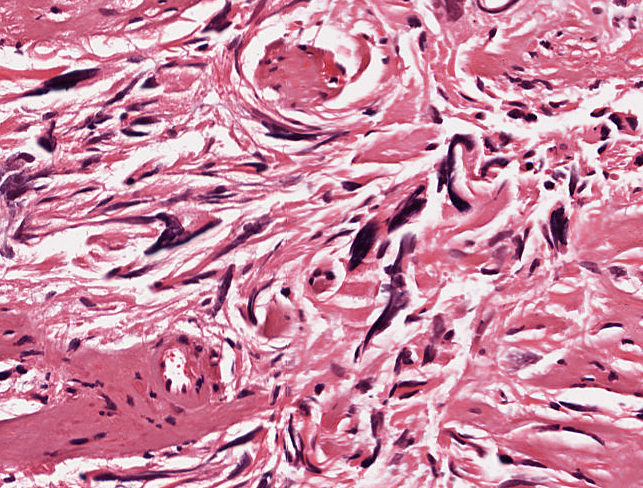
\includegraphics[width=\textwidth]{img/image1.png}
       \caption{A tissue image.}
       \label{fig:rg1}
   \end{subfigure}
   \hspace{3mm}
   \begin{subfigure}[b]{0.45\textwidth}
        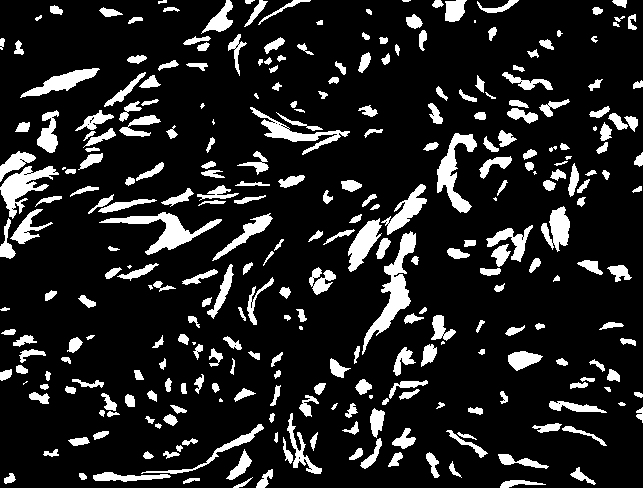
\includegraphics[width=\textwidth]{img/seg.png}
        \caption{The segmented tissue image.}
        \label{fig:rg2}
    \end{subfigure}
    \caption{An example of tissue image segmentation.}
    \label{fig:tissue}
\end{figure}

The quality of the workflow analysis is, however, dependent of the quality of the parameters values, with them described in Table \ref{tab:parameters}. Therefore, in order to improve the effectiveness of the analysis the impact of these parameters on the output of the used workflow (Figure \ref{fig:wf}) should be analyzed. This impact analysis is known as sensitivity analysis and is detailed on the following section.

\subsection{Sensitivity Analysis}

% The use of computational models to represent physical systems in order to analyze and understand such systems has become rather common in recent years. With the increase of available computational power and the continuous use of such models their complexity has only increased as well. Given that for some of these models classical mathematical analysis is unfeasible we rely on empirical investigation.

We define Sensitivity Analysis (SA) as the process of quantifying, comparing and correlating the input parameters of a workflow with the intent of quantifying the impact of each input to the final output of the workflow \cite{sa}. This process is applied on several phases of scientific research including, but not limited to model validation, parameter studies and optimization, and error estimation \cite{sa2}. The outcome of such methods, as defined in \cite{rtf2}, are statistics that quantify variance in the analysis results as well as measures such as sensitivity induces that indicate the amount of variance in the analysis results that can be attributed to individual parameters or combinations of parameters.

Usually, the computational cost for performing SA on a workflow is directly proportional to the number of parameters it has. One way to simplify the analysis on applications with large numbers of parameters, thus reducing its cost, is through the removal of parameters whose effect on the output is negligible.

This work focuses on using the already existing system, the Region Templates Framework (RTF) \cite{rtf1,rtf2}, which performs sensitivity analysis in two phases. On the first phase the 15 input parameters (Table \ref{tab:parameters}) are screened with a light, or less compute demanding,  SA method, used to remove the so called non-influential parameters from the next phase. Afterwards, a second SA method is executed on the remaining parameters, on which both first-order and high-order effects of these on the application output are quantified. This two-phase analysis is performed since the cost of more specific approaches (e.g., VBD) are prohibitively expensive.

\begin{table}[t!]
\begin{center}
%\vspace*{-2ex}
\begin{scriptsize}
\begin{tabular}{l l l l }
\hline
Parameter   & Description & Range Values      \\ \hline
%Target Image  & Normalization target image  & $[Img1,...,Img4]$     \\ \hline
B/G/R & Background detection thresholds &  $[210,220,...,240]$  \\ \hline
T1/T2  & Red blood cell thresholds & $[2.5,3.0,...,7.5]$   \\ \hline
\multirow{2}{*}{G1/G2}  & Thresholds to identify  & $[5,10,...,80]$   \\ 
   & candidate nuclei & $[2,4,...,40]$    \\ \hline
MinSize(minS)   & Candidate nuclei area threshold   & $[2,4,...,40]$    \\ \hline
MaxSize(maxS)   & Candidate nuclei area threshold & $[900,..,1500]$   \\ \hline 
MinSizePl \\ (minSPL) & Area threshold before watershed & $[5,10,...,80]$   \\ \hline
MinSizeSeg \\ (maxSS) & Area threshold in final output   & $[2,4,...,40]$    \\ \hline 
MaxSizeSeg \\ (minSS) & Area threshold in final output  & $[900,..,1500]$   \\ \hline 
FillHoles(FH)  & propagation neighborhood  & $[4$-conn$,8$-conn$]$   \\ \hline
MorphRecon(RC) & propagation neighborhood  & $[4$-conn$,8$-conn$]$   \\ \hline
Watershed(WConn)  & propagation neighborhood  & $[4$-conn$,8$-conn$]$   \\ \hline
\end{tabular}
\end{scriptsize}
\caption{Definition of parameters and range values: parameter space contains about 21 trillion points.\label{tab:parameters}}
\end{center}
\vspace{-4mm}
\end{table}

This multi-phase sensitivity analysis process is approached on \cite{sa2} as an alternative to cope with costly analysis. The application case, as seen in Figure \ref{fig:wf} uses a complex model with several input parameters (see Table \ref{tab:parameters}) and a high execution cost. As such, it is recommended that a lighter preliminary analysis method should be executed on the full range of input parameters, only to reduce these to a smaller subset of important parameters. As a way to further reduce the analysis complexity on this first screening analysis is to also drop inputs' correlation analysis. After the execution of a screening method, more complex and comprehensive analysis methods can be performed on a subset of the input parameters. The chosen SA methods for this work were Morris One-At-A-Time as a screening method \cite{moat}, and Variance-Based Decomposition as a more complete analysis.

The light SA method, Morris One-At-A-Time (MOAT) \cite{moat}, performs a series of runs of the application changing each parameter individually, while fixing the remaining parameters in a discretized parameter search space. Each of the $k$ analyzed parameters values ranges are uniformly partitioned in $p$ levels, thus resulting in a $p^k$ grid of parameter sets to be evaluated. Each evaluation output $x_i$ of the application creates a parameter elementary effect (EE), calculated as $EE_i = \frac{y(x_1, ..., x_i + \Delta_i, ..., x_k)-y(x)}{\Delta_i}$, with $y(x)$ being the application output before the parameter perturbation. In order to account for global SA the RTF uses $\Delta_i = \frac{p}{2(p-1)}$ \cite{rtf2}. The MOAT method requires $r(k+1)$ evaluations, with $r$ in the range of 5 to 15 \cite{moat2}.

The second SA method, Variance-Based Decomposition (VBD) is preferably performed after a lighter SA screening method, as the MOAT method. This is done since VBD requires $n(k+2)$ evaluations for $k$ parameters and $n$ samples, with $n$ lying in the order of thousands of executions \cite{vbd}. Thus, it is interesting to use a reduced number of parameters for feasibility reasons. VBD, unlike MOAT, discriminates the the output uncertainty effects among individual parameters (first-order) and high-order effects.

\begin{table}[]
\begin{center}
\begin{scriptsize}
\begin{tabular}{lc|lccc}
\hline
MOAT       & First-order Effect & VBD        & First-order Effect (Main) & Higher-order Effects (Total) \\
\hline
B          & -0,0108            & B          & -                  & -                    \\
G          & -0,0064            & G          & -                  & -                    \\
R          & -0,0189            & R          & -                  & -                    \\
T1         & 0,0207             & T1         & -                  & -                    \\
T2         & 0,0417             & T2         & 0,0006             & 0,0001               \\
G1         & 0,8157             & G1         & 0,2251             & 0,2371               \\
G2         & 0,9197             & G2         & 0,7305             & 0,7886               \\
MinSize    & 0,0889             & MinSize    & 0,0025             & 0,0056               \\
MaxSize    & 0,1820             & MaxSize    & 0,0150             & 0,0086               \\
MinSizePl  & 0,0341             & MinSizePl  & 0,0021             & 0,0022               \\
MinSizeSeg & -0,0155            & MinSizeSeg & -                  & -                    \\
MaxSizeSeg & -0,0184            & MaxSizeSeg & -                  & -                    \\
FillHoles  & -0,0276            & FillHoles  & -                  & -                    \\
MorphRecon & 0,1321             & MorphRecon & 0,0146             & 0,0129               \\
Watershed  & 0,0530             & Watershed  & 0,0018             & 0,0016               \\
\hline
\end{tabular}
\end{scriptsize}
\caption{Example output of a MOAT analysis with all 15 parameters and a VBD analysis with a selection of the 8 most influential parameters. The influence of a parameter is bounded in the interval [-1,1] and is proportional to its distance from 0 (i.e., 1 and -1 are the greatest values and 0 the smallest).}
\label{tab:sa-out-example}
\end{center}
\end{table}

As an example, Table \ref{tab:sa-out-example} provides the expected outcome of a two-steps SA of the used workflow. The first analysis, MOAT, is performed at an earlier moment in order to screen all parameters regarding their first-order effects or influence over the output. Afterwards, the VBD analysis can be performed with a subset of the 8 most influential parameters, yielding not only more precise first-order effect values but also a way to calculate higher-order effects through the manipulation of the {\it Total} values (e.g., for a third-order effect of T2, G1 and G2, their {\it Total} values are added together and compared with the remaining {\it Total} values).

Regardless of the SA method chosen, the use of large set of parameters (Table \ref{tab:parameters}) results in the unpractical task of performing SA on the workflow of Figure \ref{fig:wf} due to the expected cost of evaluating such large search domain. For the sake of mitigating this infeasibility issue for performing SA on the presented workflow we can execute the analysis on high-end distributed computing environments. Also, computation reuse can be employed to reduce the computational cost without the need of application specific optimizations. Both  mentioned methods are described in the next sections.

\subsection{Region Templates Framework (RTF)}

\begin{figure}[b!]
\begin{center}
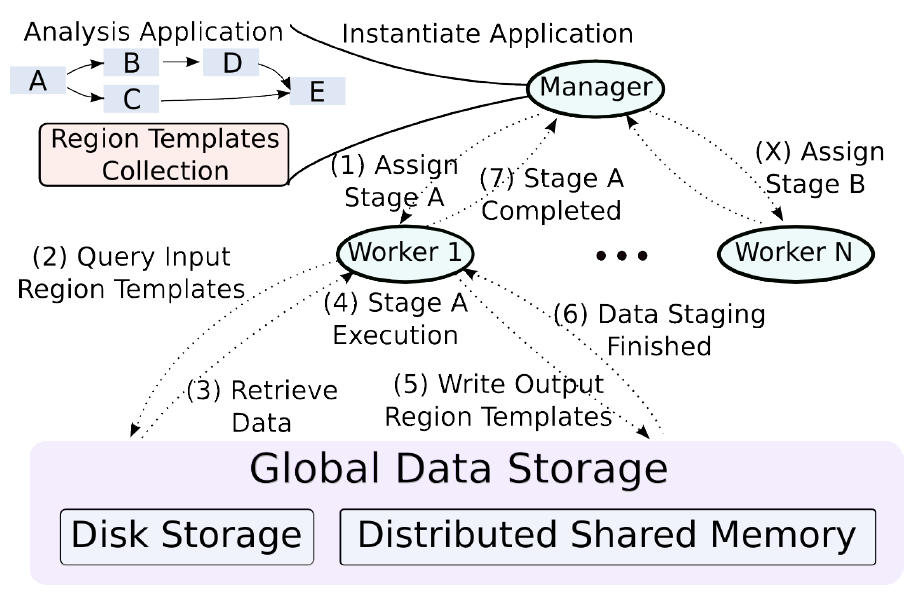
\includegraphics[width=0.95\textwidth]{img/stage_sched.png}
\caption{The main components of the Region Templates Framework, highlighting the steps of a coarse-grain stage instance execution. Image extracted from \cite{rtf1}.}
\label{fig:ss}
\end{center}
\end{figure}

The Region Template Framework (RTF) abstracts the execution of a workflow application on distributed environments \cite{rtf1}. It supports hierarchical workflows that are composed of coarse-grain stages, which in turn are composed by fine-grain tasks. The dependencies between stages, and tasks of a single stage are solved by the RTF. Given a homogeneous environment of $n$ nodes with $k$ cores each, any stage instance must be executed on a single node, with its tasks being executed on any of the $k$ cores of the same node. It is noteworthy that, not only any node can have more than one stage instance executing on it, but also, there may be  more than one task from the same stage running in parallel, given that the inter-tasks dependencies are respected.

The main components of the RTF are: the data abstraction, the runtime system, and the hierarchical data storage layer \cite{rtf1}. The runtime system consists of core functions for scheduling of application stages, transparent data movement and management via the storage layers. Figure \ref{fig:ss} shows an example of the dispatch of a stage to a worker with the data exchanges in the RTF storage layer. The RTF, with its centralized Manager, distributes the stages to be executed to Worker nodes across the network. The hierarchical workflow representation allows for different scheduling strategies to be used at each level (stage-level and task-level). Fine-grain scheduling is possible at task-level in order to also exploit variability in performance of application operations in hybrid systems. In Figure \ref{fig:ts} a stage A is sent to a worker node for execution, which tasks are scheduled locally. 

Still on the scheduler, the Manager schedules stages to Workers on a
demand-driven basis, with the Workers requesting work from the Manager until
all stages are executed. Since the Worker decides when they request more work,
a Worker can execute one or more stage at any given time instant, based on its
underlying infrastructure. Being a stage composed of tasks, these are scheduled
locally by the Worker executing them. These tasks differ in terms of data
access patterns and computation intensity, thus, attaining different speedups
if executed on co-processors or accelerators. In order to optimize the
execution of tasks a Performance Aware Task Scheduling (PATS) was implemented
\cite{rtf1,Teodoro-IPDPS2013,Teodoro:2014:CPA:2650283.2650645,cluster09george,CPE:CPE4425,doi:10.1177/1094342015594519,DBLP:journals/pc/TeodoroPKKCS13}.
With PATS, tasks are assigned to either a CPU or GPU core based on its
estimated acceleration and the current device load.

\begin{figure}[t!]
\begin{center}
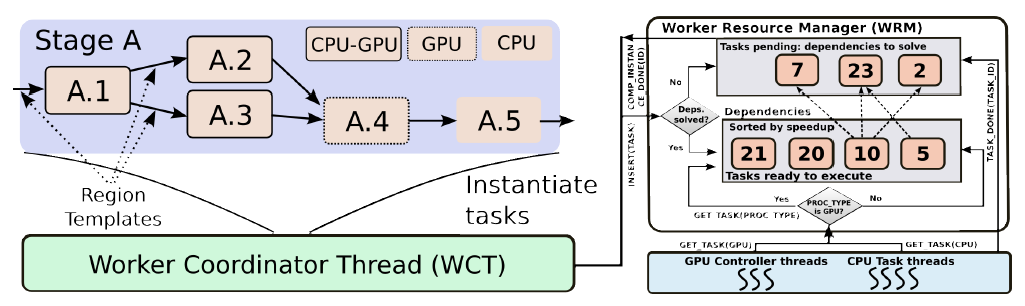
\includegraphics[width=0.95\textwidth]{img/task-sched.png}
\caption{The execution of a stage instance from the perspective of a node, showing the fine-grain tasks scheduling. Image extracted from \cite{rtf1}.}
\label{fig:ts}
\end{center}
\vspace{-4mm}
\end{figure}

On the data storage layer the Region Templates (RT) data abstraction is used to represent and interchange data (represented by the collection of objects of an application instance and the stored data of Figure \ref{fig:ss}). It consists of storage containers for data structures commonly found in applications that process data in low-dimensional spaces (1D, 2D or 3D spaces) with a temporal component. The data types include: pixels, points, arrays (e.g., images or 3D volumes), segmented and annotated objects and regions, all of which are implemented using the OpenCV \cite{opencv} library interfaces to simplify their use. A RT data instance represents a container for a region defined by a spatial and temporal bounding box. A data region object is a storage materialization of data types and stores the data elements in the region contained by a RT instance, which may have multiple data regions. 

Access to the data elements in data regions is performed through a lightweight class that encapsulates the data layout, provided by the RT library. Each data region of one or multiple RT instances can be associated with different data storage implementations, defined by the application designer. With this design  the decisions regarding data movement and placement are delegated to the runtime environment, which may use different layers of a system memory to place the data according to the workflow requirements.

% The only allowed way to express data dependencies between workflow stages and functions is through data regions. 

% Data dependencies and data exchanges between pipeline stages and functions
% within a stage are represented as data regions. Data regions consumed or
% produced by a stage or function are marked as either input, output, or input and
% output. This allows for the runtime system to manage and move the appropriate
% data used by a stage or function before it is dispatched for execution. Data
% regions at the level of a pipeline stage are defined as global data regions. A stage
% may consist of a pipeline of finer-grain functions. These functions are mapped
% to a computation node and scheduled across the CPU cores and GPUs on that
% node. Data regions generated and consumed by those functions are marked as
% local data regions. The main different between local and global data regions is
% the scope of the data region. While a local data region is only accessible within
% a particular node where the data region was created, global data regions may be
% accessed from any other computation node in the environment, e.g., by the next
% stage in the analysis pipeline that could be scheduled for execution on a different
% node. This information allows for different data storage and management
% implementations to be used in each level of the analysis pipeline, hiding the
% complexities of data management and movement decisions in hybrid computing
% systems with multiple levels of memory hierarchies.

The runtime system is implemented through a Manager-Worker execution model that combines a bag-of-tasks execution with workflows. The application Manager creates instances of coarse-grain stages, and exports the dependencies among them. These dependencies are represented as data regions to be consumed/produced by the stages. The assignment of work from the Manager to Worker nodes is performed at the granularity of a stage instance using a demand-driven mechanism, on which each Worker node independently requests stages instances from the Manager whenever it has idle resources. Each node is then responsible for fine-grain task scheduling of the received stage(s) to its local resources.

To create an application for the RTF the developer needs to provide a library of domain specific data analysis operations (in this case, microscopy image analysis) and implement a simple startup component that generates the desired workflow and starts the execution. The application developer also needs to specify a partitioning strategy for data regions encapsulated by the region templates to support parallel computation of said data regions associated with the respective region templates.

Stages of a workflow consume and produce Region Template (RT) objects, which are handled by the RTF, instead of having to read/write data directly from/to stages or disk. While the interactions between coarse-grain stages are handled by the RTF, the task of writing more complex, fine-grained, stages containing several external, domain specific, fine-grain API  calls is significantly harder for application experts. This occurs since the RTF works only with one type of task objects as its runnable interface, not providing an easy way to compose stages using fine-grain tasks. The RTF also supports efficient execution on hybrid systems equipped with CPU and accelerators (e.g, GPUs).



\subsection{Related Work on Computation Reuse}
\label{sec:reuse_intro}

The idea of work reuse, also known as value locality \cite{reuse10,reuse14}, has been employed on both the hardware and software fronts with diverse techniques, such as value prediction \cite{reuse1}, dynamic instruction reuse \cite{reuse2} and $memoization$ \cite{reuse3}, with the goal of accelerating applications through the removal of duplicated computational tasks. This concept has been used for runtime optimizations on embedded systems \cite{reuse4}, low-level encryption value generation \cite{reuse5} and even stadium designing \cite{reuse6}. In order to further analyze these existing approaches as to find desirable features that solve the problem approached in this work a qualitative analysis was performed, which is summarized on Table \ref{tab:tax}. This analysis uses taxonomic terms defined here to classify computation reuse approaches. The proposed taxonomic terminology is explained on the next section in addition to a brief analysis of each of the studied computation reuse approaches.

\subsubsection{Computation Reuse Taxonomy}

\paragraph{Implementation Level (IL)}

Computation reuse can be enforced on either {\it Software} (S) or {\it Hardware} (H) levels. By {\it Software-Level} it is meant a hardware-independent approach that can either be executed as a static analysis before the execution of any computational task, or as a runtime approach that performs computation reuse as the application is executed. Also, it is possible for computation reuse to be searched on compilation-time by a customized compiler, which is also defined as {\it Software-Level}. It is also possible for these techniques to be combined.

% {\it Software-Level} approaches provide better flexibility since the algorithm may be compiled on any architecture. However, if there is the need for a runtime service to be executed (e.g., caching), these can be more efficiently implemented on {\it Hardware-Level}. Implementing reuse on {\it Hardware-Level} also enables finer-grain tasks to be used. By using a custom compiler on {\it Software-Level} it is possible to have access to both finer-grain and coarser-grain reusable tasks. However, compilers tend to share the lack of flexibility for distinct applications of {\it Hardware-Level} approaches.

\paragraph{Application Flexibility}

Here we define the {\it Application Flexibility}(AF) of an approach as either {\it General}, {\it Partial} or {\it Domain Specific} (DS). A {\it General} approach is any that does not have domain-specific restrictions that limits or prevents its use on different domains. The flexibility of an approach can also be {\it Partial}, meaning that either some non-trivial adaptations need to be employed or that anything outside its application domain will execute rather poorly. If an approach can only be used on a rather specific environment, or under strict restrictions it is said to be a {\it Domain Specific} approach.

\paragraph{Reuse Strategy}

One of the most important computation reuse characteristics is how computation reuse opportunities are found and explored. These can be defined as {\it Predictive}, {\it Memoization} or {\it Analytic} approaches. Computation reuse can be attained through the speculative technique of {\it Value Prediction} \cite{reuse2,reuse10} with its implementations relying on a buffer that contains the results of previous instructions executions, with which the value prediction is performed.

The most common technique for computation reuse is through {\it Memoization}, which is a cache-based approach on which reusable tasks results are stored on a buffer for later reuse. It is worth noting that the stored values are used as-is, unlike with {\it Value Prediction}, which relies on the evaluation of the buffered values in order to return a reusable value. This approach has the drawback of needing a buffer structure, which increases the complexity of this kind of solution.

% being able to be implemented on either {\it Hardware-Level} or {\it Software-Level}. On {\it Hardware-Level} this buffer, or cache, is usually small since caching is expensive (both footprint and financial wise), and cannot have a flexible size. These limitations are smaller with {\it Software-Level} buffers, however, at the cost of performance. For a buffer implementation on this level a runtime system is necessary in order to keep track of all reusable results. 

%This buffer must also be much greater in size when compared with a {\it Hardware-Level} cache since its reusable tasks are of a coarser granularity, meaning that usually their input range domain is far greater than the finer-grain hardware counterpart.

The alternative to {\it Memoization} is to find all reuse opportunities in an {\it Analytic} manner. This means that the reused tasks were found {\it a priori}, instead of searching the results in a buffer as with the {\it Memoization} scheme. While this approach is considered to be the one with the least overhead, such analysis is more difficult to be achieved.

%and usually means that the domain application has some restrictions that enables its use.

\paragraph{Tasks Granularity}

Still another rather important aspect of computation reuse is the {\it Granularity} of the reusable tasks. On this work we break {\it Task Granularity} in four categories: {\it Instruction-Level} (i.e., CPU instruction), {\it Fine-Grain Subroutines}, {\it Coarse-Grain Routines} and {\it Full Application}. We differentiate {\it Fine-Grain} from {\it Coarse-Grain} tasks by their semantical meaning, and as a consequence, their overall cost. If a task is big enough to have a broader meaning (e.g., a segmentation operation) we call it a {\it Coarse-Grain Routine}. If the task is bigger than a CPU instruction but also not big enough to have a more abstract meaning (e.g., the preparation of a matrix on memory, or a set of loops on an algorithm) we define them as {\it Fine-Grain Subroutines} or tasks. Finally, some approaches may only be able to work with a {\it Full Application} execution.

The importance of the granularity for computation reuse is that it limits the maximum amount of reuse of any application. As an example we have a segmentation algorithm. If we were to break it in CPU instructions and then perform a complete search for reusability (i.e., search for all available reuse) we would attain the maximum possible reuse. However, the potential overhead for exploiting this level of reuse is high. By grouping this low-level operations into subroutines we reduce the number of tasks, making the search for reuse more feasible. This grouping would also hide some reuse opportunities, effectively reducing the reuse potential of the application. 

% Notwithstanding, this grouping into coarser-grained tasks would also make the reusable tasks more complex, meaning that they can have more possible outcomes and, as a consequence, making bigger buffers necessary for {\it Memoization}-based approaches.

\paragraph{Reusable Tasks Matching (RTM)}

An easy way to improve the reuse degree of an application is by relaxating the matching constraint for reuse. By doing this, reuse is possible even if not all tasks' parameters match, unlike the most common case on which all tasks' parameters are the {\it Same}. The obvious consequence of doing this relaxation is that the tasks' results will be different. However, some applications can deal with small imprecisions of its tasks (e.g., neural networks, multimedia applications, floating-point operations). As such, given that these partial (or {\it Similar}) matchings respect the precision necessary for these applications which can cope with such imprecisions, this strategy can improve the amount of reuse available.

%\paragraph{Task Granularity Flexibility (TGF)}

%An interesting feature proposed by two of the analyzed works \cite{reuse4,reuse9} is to have the task granularity to be adaptable to the application instance. By doing this it is possible to better deal with the trade-off of coarser vs finer task granularity. Yet, the computation reuse approaches that implement this feature had to either have a {\it Training} step or used profiling data, making them more complex to use.

\paragraph{Reuse Evaluation}

Computation reuse can be analyzed either {\it Dynamically}, at runtime, of {\it Statically} before the execution of any task. 

% Performing {\it Static} analysis incur in no runtime overhead, as opposed to a {\it Dynamic} approach. However, dynamism on computation reuse analysis is interesting for load balancing reasons.

\paragraph{Training Required (T)}

Approaches that rely on domain-specific characteristics of applications (e.g., neural networks) usually require a {\it Training} step before the reuse analysis. For these approaches it is important to be mindful of the {\it Training} cost.
% , as it is possible for it to dominate the full analysis makespan.

\paragraph{Reusability Environment Scale (RES)}

The reusable tasks scope is defined here as the {\it Reusability Environment Scale}. The tasks can be reusable among a {\it Distributed} (D) environment of computing nodes or reused only {\it Locally} (L). 

% For tasks to be able to only be reused {\it Locally} is very restrictive, since the maximum scale of the application becomes limited rather quickly. 

%For the large scale of Sensitivity Analysis for Microscopy Image Segmentation, a {\it Local} reuse approach is impractical.

%\paragraph{Objective}

%The final analyzed feature is the {\it Objective} of the computation reuse approach. It is most common for computation reuse to focus on reducing the {\it Makespan} of the application. Nevertheless, some applications focused on optimizing the overall {\it Energetic Cost} of the application. It is worth noting that while these two {\it Objectives} are interlinked (i.e., by optimizing one, the other is very likely to improve as well), optimizing there are cases on which they are contrasting objectives (e.g., assuming a {\it Distributed} reuse application on which maximum reuse means serialization, to optimize the {\it Makespan} some reuse opportunities should be ignored in order to balance the load between the execution nodes).

\subsubsection{Related Work Analysis}

Sodani and Sohi \cite{reuse2} motivate their work by drawing a parallel of a computation \textit{reuse buffer} used to optimize instruction execution with memory cache used to optimize memory access instructions. Their approach aims to reduce computational cost through reuse by (i) ending the instruction pipeline earlier, thus also reducing resources conflicts, and (ii) by breaking dependencies of later instructions, which can be executed earlier since the necessary inputs are already present. They initially proposed their \textit{reuse buffer} as a way to reduce branch misprediction penalties. However, the effectiveness of this approach proved itself much more powerful since the reuse frequency of other, more generic, types of instructions also proved to be high. Their implementation focus on adding a \textit{reuse buffer} to any generic dynamically-scheduled superscalar processor, using one of the three instruction reuse schemes proposed by them. 

The approach on \cite{reuse2} can be used for any application domain while also being exposed to the largest possible amount of reuse opportunities. Their incorporation of the \textit{reuse buffer} in a superscalar processor is done without impacting the pipeline  critical path, thus having no negative impact on non-reused instructions. Nevertheless, the efficiency of all instruction reuse schemes are heavily reliant on the buffer size. Although the used buffer sizes tested by them are small, this dependency is a limiting factor for the approach since smaller buffers means less reuse opportunities. Finally, the use of a hardware-based approach limits its use even further given the difficulty to design a processor for this sole purpose.

The work on \cite{reuse3}, similarly to \cite{reuse2}, also uses hardware-level $memoization$, but this time with a subset of operations called \textit{trivial computation}. These are potentially complex operations that are trivialized by simple operands (e.g., integer division by two). This strategy greatly simplifies the reuse protocol (i.e., whether an instruction is reused, insertion and replacement policies) at the cost of reuse opportunities. The speedups achieved by this approach were only significant when the application was favorable to the reuse strategy (e.g., Ackerman-like applications with huge amounts of trivial operations, or floating-point-intensive programs, which have naturally long-latency instructions). The same limitations of \cite{reuse2} were present here as well.

Wang and Raghunathan \cite{reuse4} attempt to reduce the energetic cost of embedded software on battery-powered devices through a profiling-based reuse technique with a $memoization$ structure. Some interesting discussions risen in their work regard reusable tasks granularity and the limitations of hardware-based reuse. Hardware implementations of computation reuse are usually complex, and the use of overly fine-grained operations for reuse may yield little or negative speedups given the overhead of $memoization$ caches.

The methodology of \cite{reuse4} consists on profiling an application, generating \textit{computation reuse regions}, setting the software cache configuration, evaluating the energy expenditure and then doing it all over again until a good enough solution is found. Only then, the optimized application is sent to production. The concept of flexible \textit{computation reuse regions} is very powerful since it makes the application more domain-independent while also optimizing the granularity of the reuse for any application instance. Their automated software cache configuration is also interesting since any $memoization$-based technique is heavily reliant on its size and performance.

Unfortunately \cite{reuse4} do not specify the cost of profiling (since for the test environment the typical input traces of the selected benchmarks were already available), nor the cost of configuring the \textit{computation reuse regions} and the software cache. Regardless, this approach, while presenting the concepts of flexible granularity and automatic software cache configuration / optimization, cannot be recommended for large-scale workflow execution given its unknown-cost training step. Also, in order to distribute the computation reuse, the software cache used by it needs to be re-thought to be compatible with this paradigm.

It is brought to our attention on \cite{reuse5} the cost of two-party secure-function evaluation (SFE) and the tendency to offload these operations from resource-constrained devices to outside servers. In order to reduce the computational cost of these SFE operations as well as bandwidth requirements, a system on which state is retained as to later be reused was implemented. The reusable encrypted values can be used by a number of clients on a distributed setting, originating from a centralized server node that implements a $memoization$ buffer.

Although \cite{reuse5} is the first approach to enable computation reuse to be done in a distributed environment, the encrypted values buffer is a bottleneck for the approach scalability. In order to remove this bottleneck, the buffer can be distributed among server nodes, which has as a consequence either (i) the buffers are coherent, and as such the servers need to keep trading messages to enforce it, or (ii) the buffers are not coherent and thus the reuse potential is reduced. Finally, this approach is only partially applicable for different application domains since the granularity of the reused tasks must be rather coarse in order to achieve good speedups. This happens because the of the big overhead of reusing encrypted values.

Approach \cite{reuse7} also works with distributable reusable values, but this time with  bioinformatics applications, which are known to be computationally expensive. The granularity of reusable tasks is even coarser, being able to perform full end-to-end reuse of workflows. When comparing with \cite{reuse5}, \cite{reuse7} has the same limitations given its $memoization$-based approach.

On \cite{reuse8} Santos and Santos propose the use of a software-level runtime buffer system to cache and then reuse energy evaluations for predicting the native conformation of proteins. The domain-specific application relies on a genetic algorithm, and as such, their approach is tailored for this single application. A similar approach is the one of Yasoubi et al. \cite{reuse9}, regarding the use of $memoization$-based computation reuse, optimized for a specific domain, which is neural networks on this case.

Yasoubi et al. \cite{reuse9} propose an offload hardware accelerator that uses clustered groups of neurons that maximize the expected computation reuse when executing the application. It is worth noting that the clustering is done by a k-means algorithm on software level. The reusable tasks are hardware-level multiplication instructions that, given the multi-processing-unit (multi-PU) architecture, disable PUs that perform repetitive operations, thus reducing the power consumption.

The work of Connors and W.Hwu \cite{reuse10} exploit value locality through the combination of a hardware buffer, an instruction set for representing different-sized reusable computational tasks and a profile-guided compiler that groups instructions into reusable tasks as to optimize their granularity. This approach was implemented as a way to extend hardware-only-based reuse approaches while solving the limitation of instruction-level reusable tasks granularity. Again, the use of dynamically-sized reusable tasks makes the approach more flexible to different domains of applications while optimizing the reusable tasks granularity for each application instance. However, in order to implement this feature the approach on \cite{reuse10} limits itself by needing a complex hardware and compiler implementation and profiling information on the domain-specific application.

Álvarez et al. \cite{reuse11} focus on reducing the power consumption of low-end and/or mobile devices by applying computation reuse on multimedia applications. This is done by exploiting the imprecision tolerance of multimedia floating-point operations at hardware-level to reuse tasks that are similar enough, thus increasing the amount of attainable computation reuse. Nonetheless, this ``similar enough'' strategy limits the usability of this approach to multimedia applications, or applications which have a large number of floating-point reusable operations. The same is true for approach \cite{reuse13}, which in turn proposes a more generic implementation that was not tailored for multimedia applications.

The first analytic computation reuse method is presented by Xu et al., on \cite{reuse12}. On their work they propose a framework for Isogeometric Analysis (IGA) that reuse matrix calculations. The reuse operations were statically analyzed \textit{a priori} and are specific of IGA, meaning that this approach, although having good speedups, cannot be applied for other application domains.

Lepak and Lipasti \cite{reuse14} propose reuse of memory load instructions. This is done through the characterization of value locality for memory instructions and the implementations of two reuse protocols for both uniprocessed and multiprocessed environments. For uniprocessed systems reuse can be attained by either analyzing the value locality of specific instructions (based on the program structure), or the locality of a particular memory address (message-passing locality). Furthermore, they define \textit{silent stores} as stores operations that do not change the system state (i.e., the written value is the same as the one previously present on memory). Given some statistical analysis of how many \textit{silent stores} are on selected benchmarks, they set an ideal maximum reuse possible to be achieved and, through their proposed protocols, aim to get as close as possible to these values.

\begin{table}[t!]
\begin{center}
\vspace*{-2ex}
\begin{scriptsize}
\begin{tabular}{ccccccccc}
\toprule

Reference       & IL         & AF & Reuse Strat. & Tasks Granularity                                & RTM & Reuse Eval. & T & RES \\

\midrule

\cite{reuse1} & H            & Flexible                   & Predictive          & Instruction-Level                                & Same       & Dynamic          & No             & L   \\
\cite{reuse2} & H            & Flexible                   & Memoization         & Instruction-Level                                & Same       & Dynamic          & No             & L   \\
\cite{reuse3} & H            & Flexible                   & Memoization         & \makecell{Instruction-Level \\ Trivial Operations}             & Same       & Dynamic          & No             & L   \\
\cite{reuse4} & S            & Flexible                   & \makecell{Analytic + \\ Memoization}  & \makecell{Fine-Grain \\ Regions of Code} & Same       & Static           & Yes            & L   \\
\cite{reuse5} & S            & Partial                 & Memoization         & Coarse-Grain                          & Same       & Dynamic          & No             & D   \\
\cite{reuse7} & S            & Flexible                   & Memoization         & Full Application                                  & Same       & Dynamic          & No           & D  \\
\cite{reuse8} & S            & DS                    & Memoization         & Coarse-Grain          & Same       & Dynamic          & No             & L   \\
\cite{reuse9}       & H+S & DS                    & Memoization         & \makecell{Instruction-Level \\ Complex Operations} & Similar             & Dynamic          & Yes            & L   \\
\cite{reuse10}       & H+S & Partial        & Memoization         & \makecell{Instruction-Level + \\ Fine-Grain \\ Regions of Code} & Same       & \makecell{Static + \\ Dynamic}          & Yes     & L  \\
\cite{reuse11}       & H            & Partial & Memoization         & \makecell{Instruction-Level \\ Floating-Point \\ Operations}     & Similar             & Dynamic          & No             & L   \\
\cite{reuse12}       & S            & DS                    & Analytic            & Coarse-Grain                          & Same       & Dynamic          & No             & L         \\
\cite{reuse13}       & H            & Partial       & Memoization         & \makecell{Instruction-Level \\ Floating-Point \\ Operations}     & Similar             & Dynamic          & No             & L                 \\
\cite{reuse14}       & H            & Flexible                   & Memoization         & Instruction-Level                                & Same       & Static          & No             & L  \\
\midrule

Our Work       & S            & Partial                & Analytic            & \makecell{Coarse-Grain \\ and Fine-Grain}        & Same       & Static           & No             & D \\

\bottomrule

\end{tabular}
\end{scriptsize}
\caption{Taxonomic evaluation of computation reuse approaches. Implementation Level (IL): Hardware (H) or Software (S). Application Flexibility (AF): Flexible, Partial or Domain Specific (DS). Reuse Strategy: Predictive, Memoization or Analytic. Task Granularity: Instruction-Level, Fine-Grain, Coarse-grain or Full Application. Reusable Tasks Matching: Same or Similar. Reuse Evaluation: Static or Dynamic. Needs Training Step (T). Reusability Environment Scale (RES): Local (L) or Distributed(D).\label{tab:tax}}
\end{center}
\vspace{-4mm}
\end{table}

Since none of the previous applications is either compatible or flexible enough to work on the large scale bioinformatics workflows application domain, this work proposes a novel approach to computation reuse. The proposed approach works with software-level reuse, since it is being implemented on top of the RTF. Also, given that this application is supposed to be executed on a large-scale cluster environment, hardware-based approaches are impractical. Moreover, the runtime system must be light in order to execute on a large-scale distributed environment, thus making the use of $memoization$ impractical. Given that the application uses hierarchical workflows, any applications of other domains need to be converted to workflows in order to be executed by our approach, slightly impacting the application domain flexibility. Finally, computation reuse is achievable by a static analytic analysis of reuse before the execution of any task, thus removing any distribution limitations as long as the reuse analysis can be performed quickly.

% All of those approaches can be placed into one of two categories, hardware-level or software-level reuse. This work focus on the second type since hardware-level reuse requires specific hardware designing, which is not the target of this work.

% On software-level reuse two main techniques were noticed, (i) reuse based on pre-execution profiling and (ii) $memoization$ of recurrent tasks. The first method \cite{reuse4}, although efficient, is rather application dependent and incurs in a pre-execution training step, which could be unfeasible to implement for SA applications given the size of the parameters set domain.

% The other common approach is through caching of results of selected executions \cite{reuse3, reuse7,reuse8} named $memoization$. This method can virtually be used for any application domain. However, increases in the number of reuse opportunities available are achieved through either more domain-specific selection methods or by increasing the amount of memorized results. Also, in order to reduce the overhead of searching for reusable tasks results, higher-level operations ought to be used, effectively reducing the potential of reuse. Taking into account the granularity of the fine-grain task of the workflow used on this work and the scale of the number of tasks, the storage of this many results would be impractical. Finally, while the use of $memoization$ can easily be brought to multiprocessed environments through the addition of parallel control structures (e.g., locks), when we attempt to bring this approach to a distributed environment there is an additional overhead for coherence enforcement, which can be hard to scale.


% On \cite{reuse2} Sodani and Sohi implement a hardware-level \textit{reuse buffer} for some instructions, which if an operation under execution is found, its execution can then be finished and the buffered result be returned. By doing this, Sodani and Sohi claim to have cut down the resources required to execute some instructions while also reducing the length of critical path of some operations. A similar but distinct hardware-level buffer is proposed on \cite{reuse3} for arithmetic operations.

% On software level Wang and Raghunathan propose on \cite{reuse4} the use of computation reuse in order to make embedded applications more energy efficient. This is done by profiling the target application, grouping operations into reuse regions, generating a software-level cache and then doing this process over with new execution data in a feedback loop. This approach draws some similarities with \cite{reuse5}, in the sense that low-level software operations are reused through the caching of some results.

% Still on software level, but on a higher level of abstraction, \cite{reuse7,reuse8} proposes the application of computation reuse on high-level complex operations or functions. On \cite{reuse7}, complete analysis applications for genetic research can be reused if all input parameters match. This is done with the goal of reproducibility. Finally, \cite{reuse8} analyses reusing fitness calculation results for genetic algorithms applied to protein folding applications. Both approaches use a software-level cache to store reusable results.

% When analyzing the above approaches for computation reuse and trying to apply their concepts to our domain of SA, any hardware-level proposal cannot be used. Their use would unnecessarily increase the complexity of the application while making any type of parallelism hard to achieve. Regarding \cite{reuse4} software-level approach, even a simple segmentation analysis application is too expensive for profiling. Moreover, while the flexibility of runtime operation grouping is desirable, the image segmentation analysis workflow used in this work is simple enough to be efficiently analyzed manually. Finally, regardless the level on which computation reuse is applied, caching approaches add an operations layer which needs to be optimized to the specific hardware environment on which it is being executed (e.g., the number of cache levels, cache size and number of blocks, replacement policy). This layer, while being easily implemented for serialized applications can become rather difficult very quickly for distributed applications, on which there needs to be a sense of global coherence among computing nodes. Given these problems, simpler and lighter approaches are required for the proposed computation reuse on SA applications on multiprocessed distributed environments.

% Given that any approach for computation reuse is also defined by the level of abstraction of the analyzed tasks, it is worth noting that higher-level task reuse (or coarse-grain task reuse) is considerably easier to implement since the granularity of coarse-grain tasks incur in more expensive tasks, and thus resulting in less inner-task communication overhead. Also, working on the coarse-grain granularity level prevents the seizing of partial reuse opportunities.

% Finer-grain task reuse can hence explore the missed opportunity of partial reusable coarse-grain tasks, since only the common portion can be reused. This approach is however much more difficult to cope with since the communication overhead between merged tasks is more significant given that fine-grain tasks are computationally less expensive. 

% Also, for the RTF environment performing stage merging indiscriminately can have a toll on parallelism. This is most prominently seen when analyzing a set of workflows which all of its stages instances have some minor degree of reuse opportunities among themselves. By attempting to maximize the reuse of such stages instances we would at the same time minimize the overall computational cost of the analysis and serialize the execution of the stages to a single node. 

% With these characteristics for fine-grain reuse none of the previous analyzed works can be efficiently employed to solve this problem. With that, this work proposes a static reuse analysis, done before the execution of any task. With this tactic there is no need for any sort of caching systems. Moreover, the results of most of the tasks are images, what makes the storage of such data impracticable since the cost of storaging these images is generally greater than the cost of executing a fine-grain task. At last, the a static reuse analysis tactic is compatible with distributed environments since it requires no additional communication between worker nodes. 

